\documentclass[tikz,border=2pt]{standalone}
\renewcommand{\familydefault}{\sfdefault}
\usetikzlibrary{arrows.meta,calc,positioning}
\tikzset{every picture/.style={line width=1pt, >=Stealth},
         hl/.style={fill=black, fill opacity=0.12, text opacity=1}}
\begin{document}
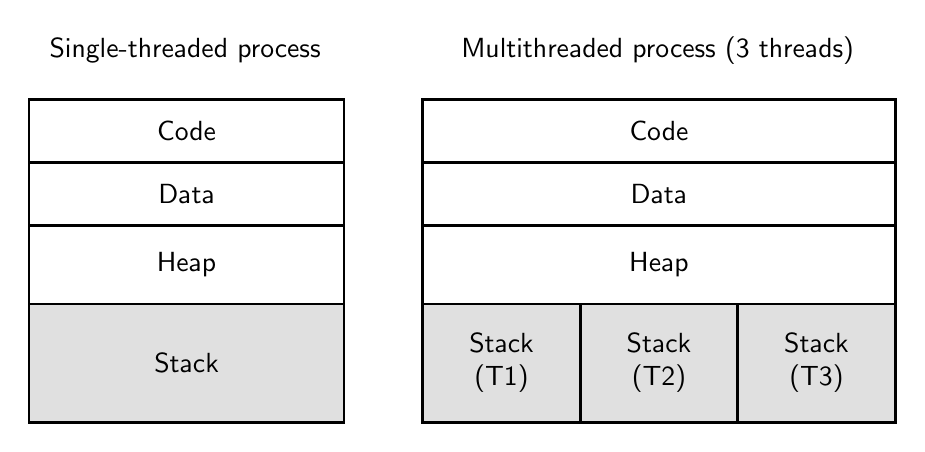
\begin{tikzpicture}[region/.style={draw, minimum height=0.8cm}]
  % Threads share code, data, and heap; each thread has its own stack.
  \foreach \x/\w/\title in {0/4/Single-threaded process, 5/6/Multithreaded process (3 threads)} {
    \node at (\x + \w/2, 0.6) {\title};
    \node[region, minimum width=\w cm, anchor=north west] at (\x, 0) {Code};
    \node[region, minimum width=\w cm, anchor=north west] at (\x, -0.8) {Data};
    \node[region, minimum width=\w cm, minimum height=1cm, anchor=north west] at (\x, -1.6) {Heap};
  }
  \node[region, hl, minimum width=4cm, minimum height=1.5cm, anchor=north west] at (0, -2.6) {Stack};
  \foreach \t in {1, 2, 3}
    \node[region, hl, minimum width=2cm, minimum height=1.5cm, anchor=north west, align=center] at (5 + 2*\t - 2, -2.6) {Stack \\ (T\t)};
\end{tikzpicture}
\end{document}
